% --------------------------------------------------------------------------- %
% --------------------------------------------------------------------------- %
\chapter{Same-Sign Dilepton Signature}
\label {ch:ss}

As discussed in Section~\ref{sec:intro_ss}, there are many models that predict
same-sign dileptons, hadronic jets, and \met. In order to determine if there is
an excess of events, an accurate prediction of the expected background to this
signature must be performed. In this chapter, a brief description will be given
for the SM background processes that give genuine same-sign dileptons that are
both prompt and isolated (rare SM). These constitute an irreducible background
to the analysis that must be accounted for. These processes are discussed in
Section~\ref{sec:ss_rare}.

The other two major sources of background include objects mis-identified as
selected leptons (fakes) and leptons with a mis-identified charge and from
genuine opposite-sign pairs (charge flips). These backgrounds sources are a
result of the failure of the selection to properly classify these events and
these sources are discussed in Section~\ref{sec:ss_bkgd}.

% --------------------------------------------------------------------------- %
% --------------------------------------------------------------------------- %
\section{Rare Standard Model Processes}
\label{sec:ss_rare}
% --------------------------------------------------------------------------- %
% --------------------------------------------------------------------------- %

As discussed previously, the main source of irreducible background is processes
that produced genuine prompt and isolated same-sign leptons in the final state.
In this section, we provide a brief description of the main processes that the
SM predicts and are included in this analysis.

% --------------------------------------------------------------------------- %
\subsection{Top Processes}
\label{sec:ss_rare_top}
% --------------------------------------------------------------------------- %

Processes involving top production with an associated gauge boson is are a
significant source of same-sign dileptons. This can be seen by the example Feynman
diagram shown in Figure \ref{fig:feyn_ttw}.
% --------------------------------------------------------------------------- %
\begin{figure}[!htb]
\begin{center}
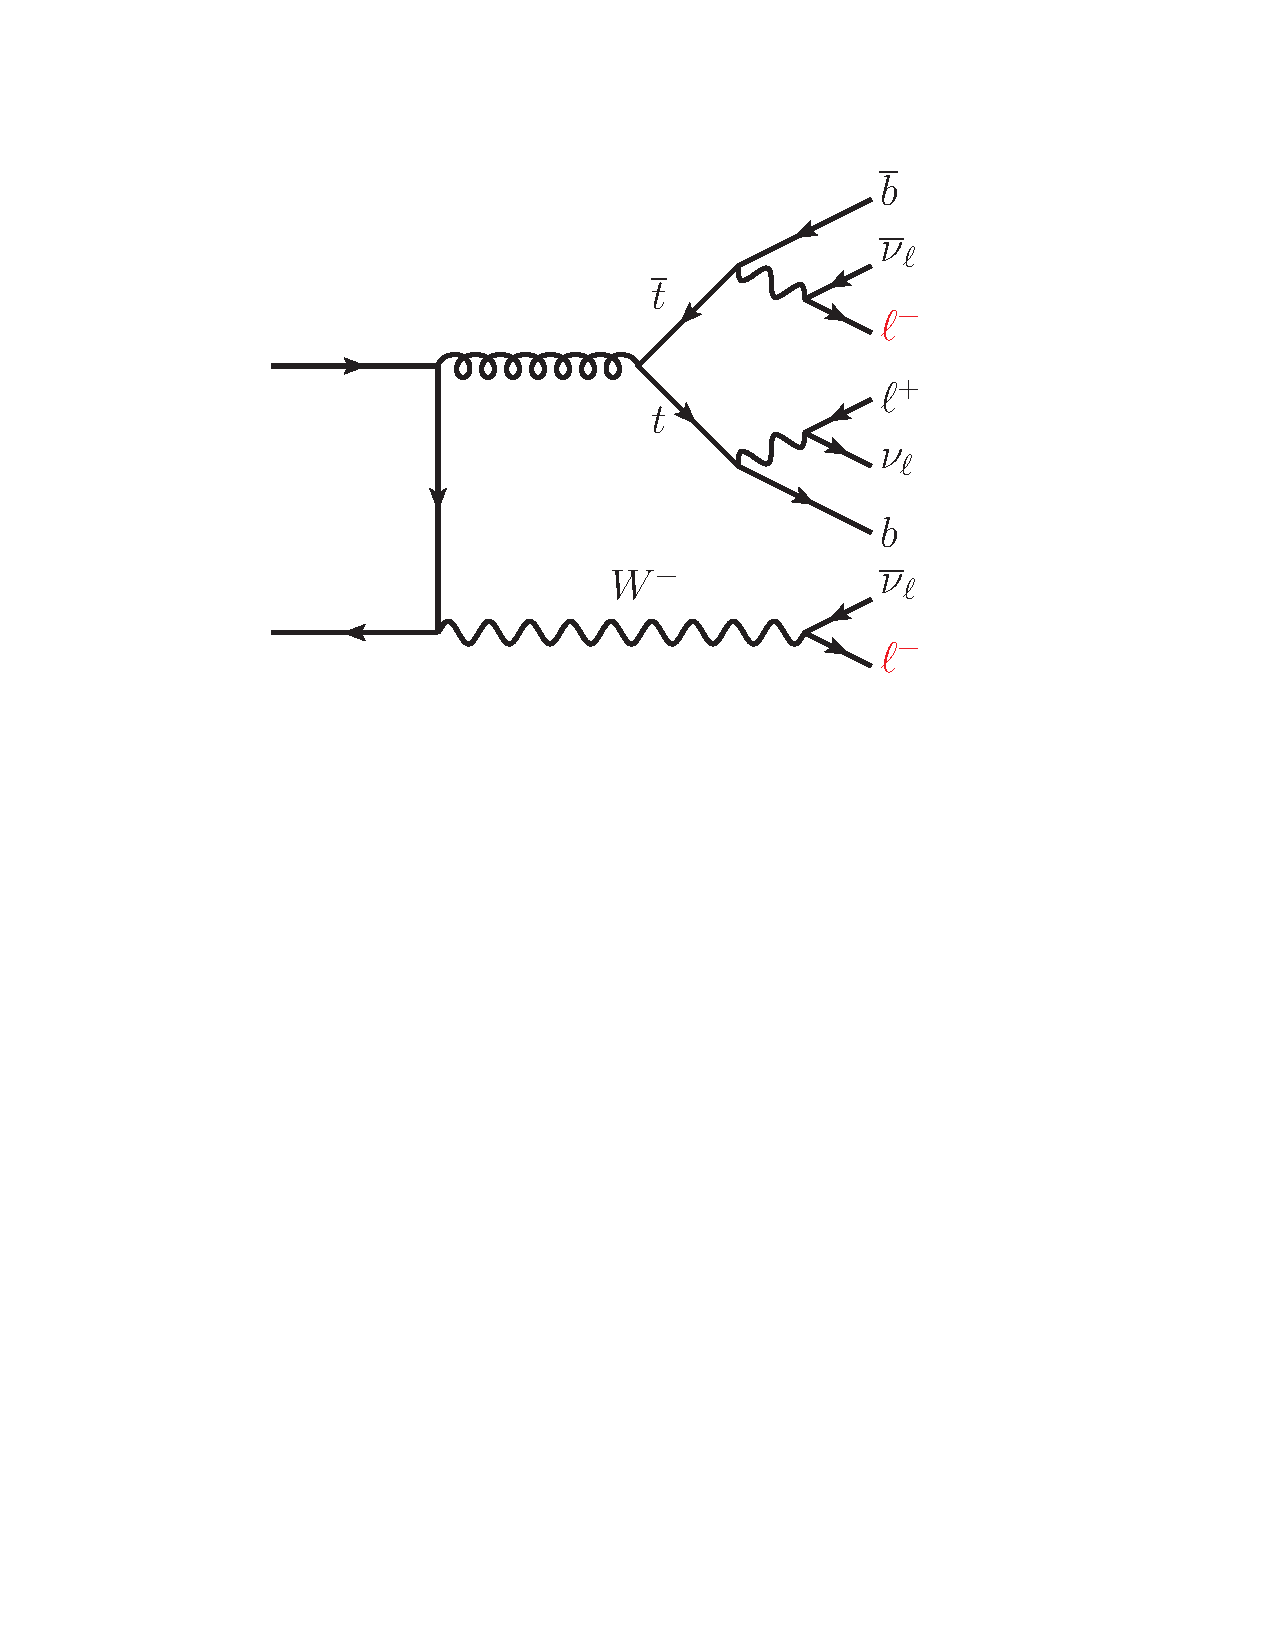
\includegraphics[width=0.8\textwidth, clip = true, trim = 1in 6.5in 1in 1in]{ttw.pdf}
\caption[Feynman diagram for \ttW]
{\label{fig:feyn_ttw}
Example leading order Feynman diagram for $pp \to \ttW \to 3\ell\nu + X$.
}
\end{center}
\end{figure}
% --------------------------------------------------------------------------- %
Top processes that are considered in this analysis are listed below:
\begin{itemize}
\item \ttW: The \W decays leptonically and the top quark with the same charge as the \W also decays leptonically ($t \to \ell^{\pm}\nu b$ and $W^{\pm} \to \ell^{\pm}\nu$).
\item \ttZ: The \Z decays leptonically and at least one of the top quarks also decays leptonically ($t \to \ell^{\pm}\nu b$ and \Zlplm).
\item \ttG: The $\gamma$ decays leptonically and at least one of the top quarks also decays leptonically ($t \to \ell^{\pm}\nu b$ and \Glplm).
\item \tbZ: The \Z decays leptonically and the top quarks also decays leptonically ($t\bar{b} \to \ell^-\nu \bar{b}$ and \Zlplm).
\item \ttWW: At least one of the \W's decay leptonically and one of the top quarks with the same sign also decays leptonically ($t \to \ell^{\pm}\nu b$ and $W^{\pm} \to \ell^{\pm}\nu$).
\end{itemize}

% --------------------------------------------------------------------------- %
\subsection{Two Gauge Boson Processes}
\label{sec:ss_rare_diboson}
% --------------------------------------------------------------------------- %
 
Processes involving the production of two electroweak bosons in the same event
can easily produce same-sign leptons. What makes them rare is their actual
production is quite low due to the mass of these bosons. A typical
example can be seen from the Feynman diagram shown in Figure~\ref{fig:feyn_wz}
below:
% --------------------------------------------------------------------------- %
\begin{figure}[!htb]
\begin{center}
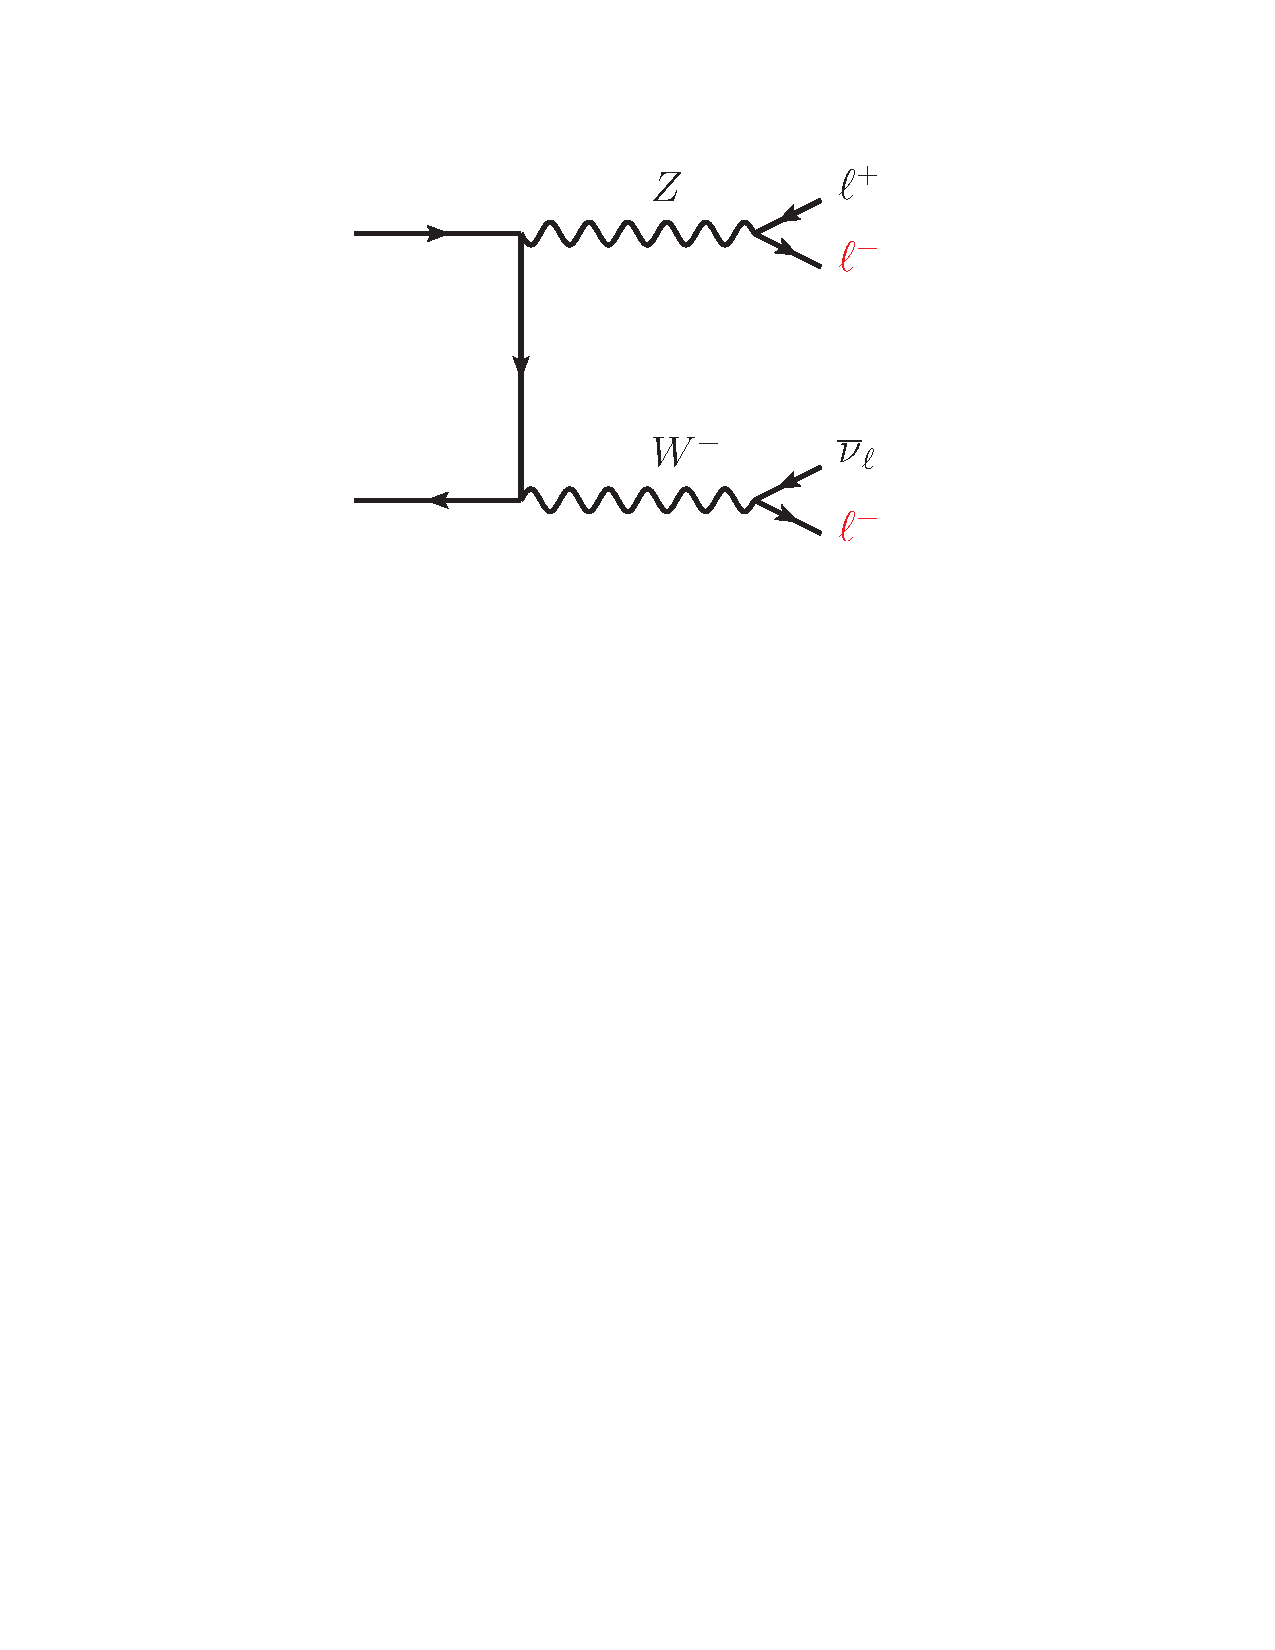
\includegraphics[width=0.8\textwidth, clip = true, trim = 1in 7.0in 1in 1in]{wz.pdf}
\caption[Feynman diagram for \WZ]
{\label{fig:feyn_wz}
Example leading order Feynman diagram for $pp \to \WZ \to 3\ell\nu + X$.
}
\end{center}
\end{figure}
% --------------------------------------------------------------------------- %
Processes than involve diboson production considered in this analysis are
listed below:
\begin{itemize}
\item \Wgamma: The $W$ and $\gamma$ decay leptonically ($W^{\pm} \to \ell^{\pm}\nu$ and $\Glplm$).
\item \WZ: The $W$ and $Z$ decay leptonically ($W^{\pm} \to \ell^{\pm}\nu$ and $\Zlplm$).
\item \ZZ: Both $Z$'s decay leptonically ($2 \times \Zlplm$).
\end{itemize}
 
% --------------------------------------------------------------------------- %
\subsection{Triple Gauge Boson Processes}
\label{sec:ss_rare_triboson}
% --------------------------------------------------------------------------- %

Processes involving the production of three electroweak bosons in the same
event can easily produce same-sign leptons. Producing three gauge boson is
considerably suppressed with respect to processes with two bosons since this
requires even more energy to produce due to the additional mass of the extra
boson. A typical example can be seen from the Feynman diagram shown in Figure
\ref{fig:feyn_vvv}.
% --------------------------------------------------------------------------- %
\begin{figure}[tbhp]
\begin{center}
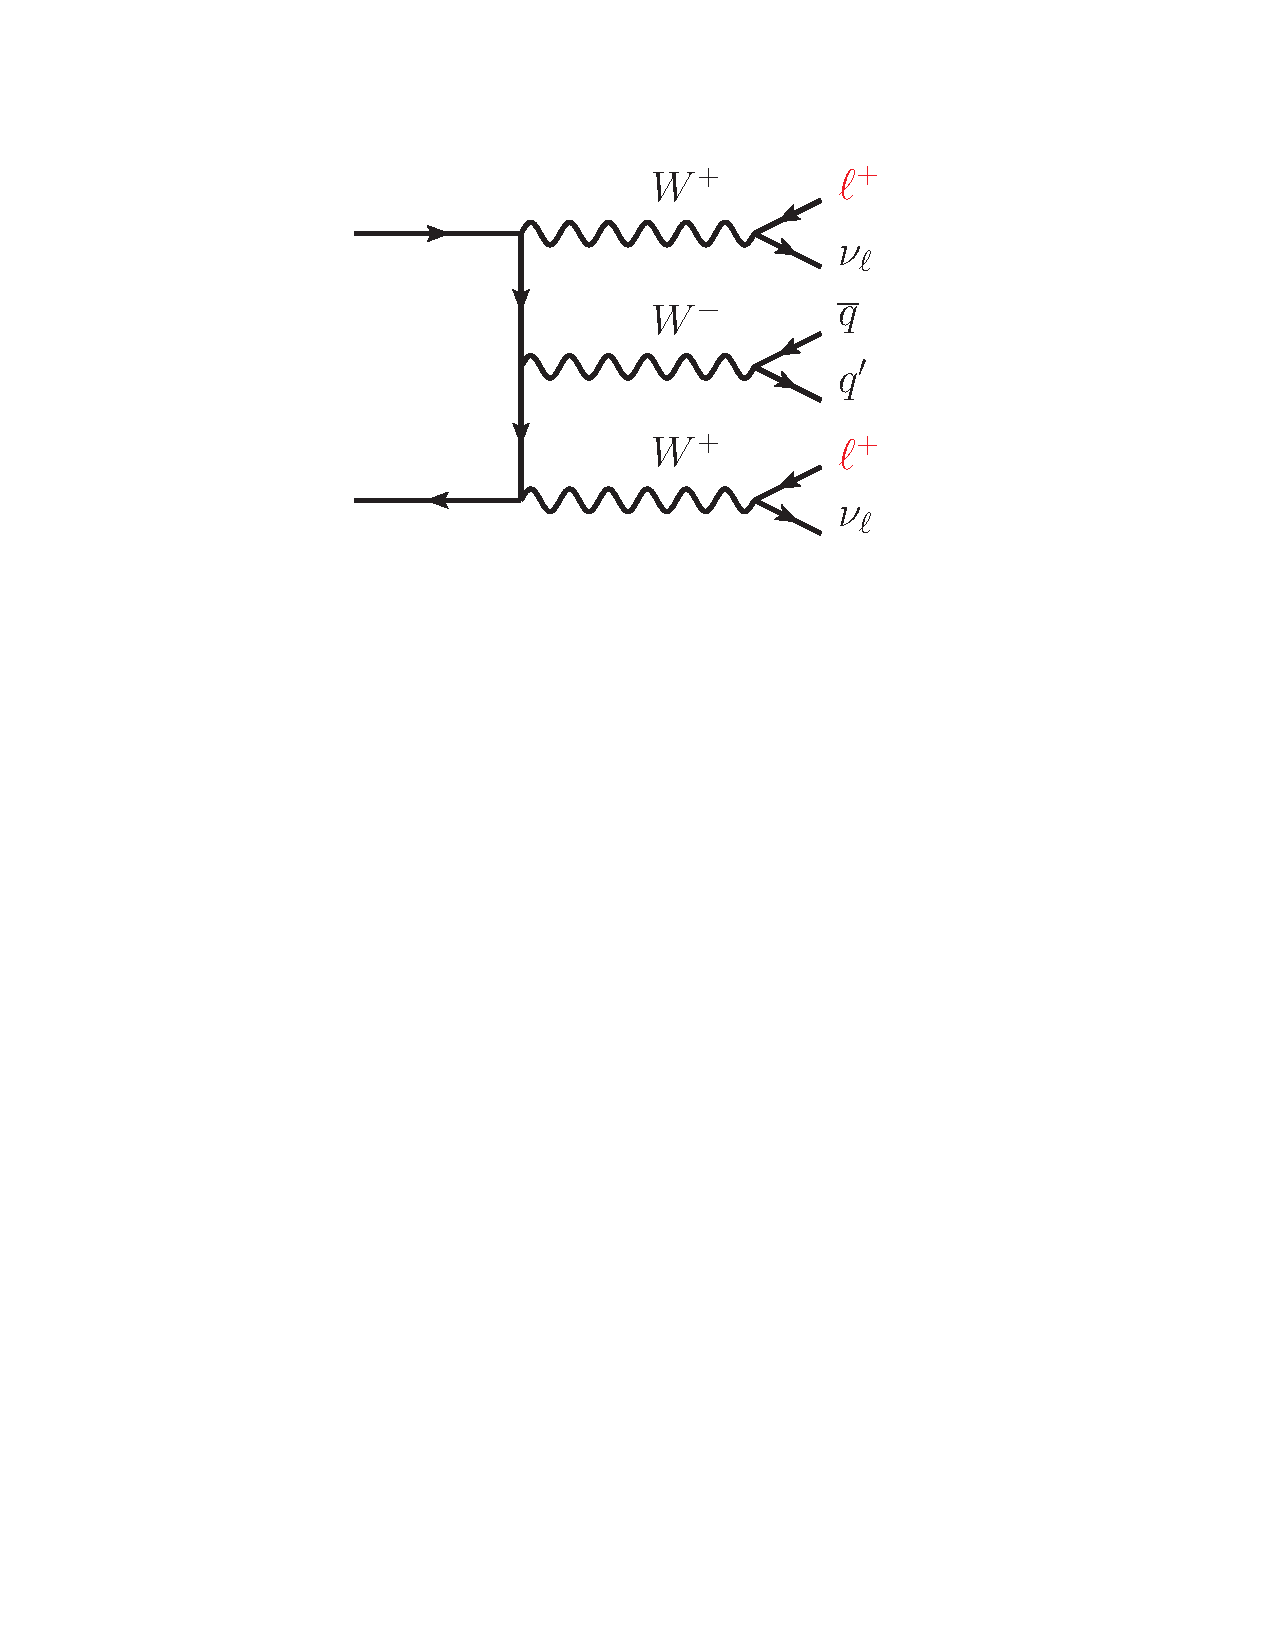
\includegraphics[width=0.8\textwidth, clip = true, trim = 1in 7.0in 1in 1in]{www.pdf}
\caption[Feynman diagram for \WZ]
{\label{fig:feyn_vvv}
Example leading order Feynman diagram for $pp \to \WWW$.
}
\end{center}
\end{figure}
% --------------------------------------------------------------------------- %
Processes that involve triboson production considered in this analysis are
listed below:
\begin{itemize}
\item \WWG: One or both $W$ bosons decay leptonically and the $\gamma$ decays leptonically ($\Wpmlpmnu$ and $\Glplm$).
\item \WWW: Two of the $W$ bosons with the same sign decay leptonically ($2 \times W^{+} \to \ell^{+}\nu_{\ell}$ or the charge conjugate).
\item \WWZ: One of the $W$ bosons and the $Z$ boson decay leptonically ($\Wpmlpmnu$ and $\Zlplm$).
\item \WZZ: Either the $W$ boson and at least one of the $Z$ bosons decay leptonically or both $Z$ bosons decay leptonically ($\Wpmlpmnu$ and at least one $\Zlplm$ or $2 \times \Zlplm$).
\item \ZZZ: At least two of the $Z$ bosons decay leptonically ($2\ \rm{or}\ 3 \times \Zlplm$).
\end{itemize}

% --------------------------------------------------------------------------- %
\subsection{Higgs Boson Processes}
\label{sec:ss_rare_higgs}
% --------------------------------------------------------------------------- %

Processes involving the Higgs boson production in conjunction with a $W$ or $Z$ boson or a top quark pair.
The Higgs can decay to W or Z bosons or tau leptons which can lead to same sign dileptons.
A typical example can be seen from the Feynman diagram shown in Figure \ref{fig:feyn_higgs} below:
% --------------------------------------------------------------------------- %
\begin{figure}[tbhp]
\begin{center}
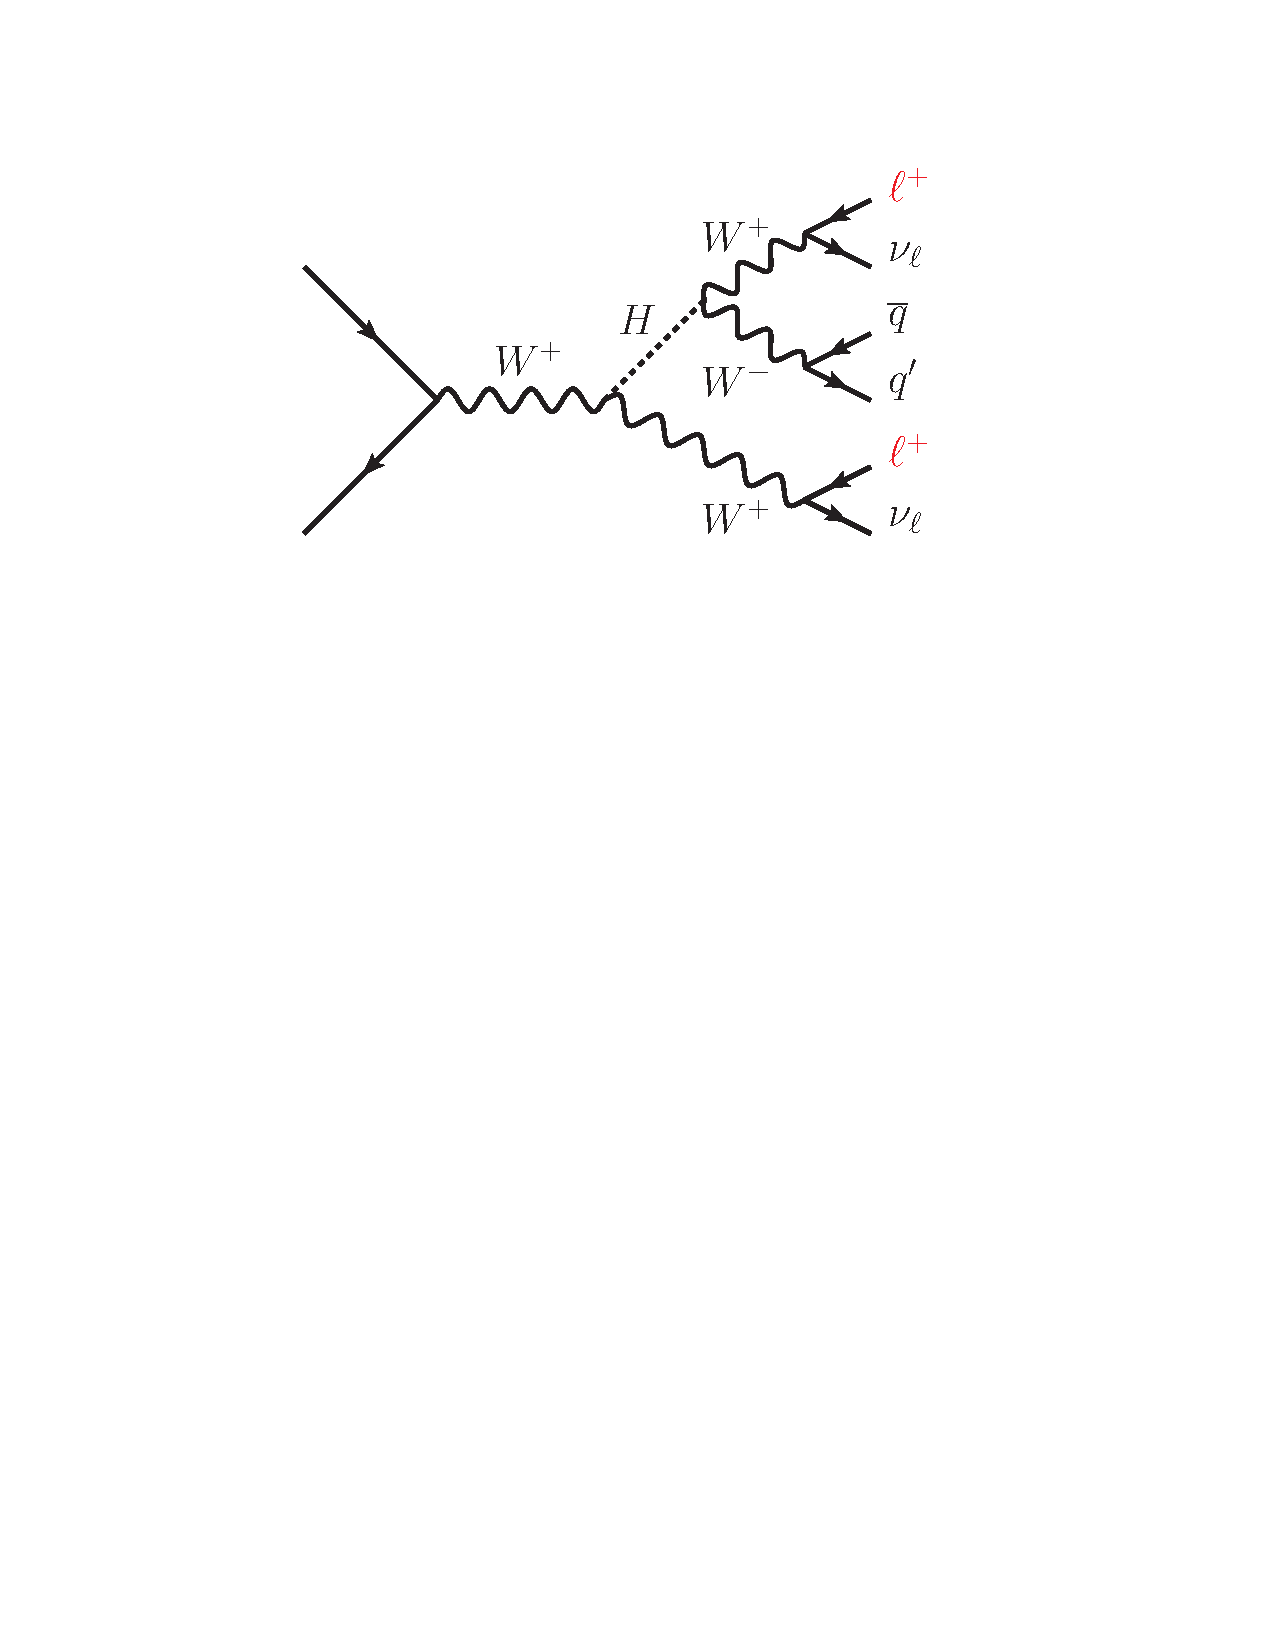
\includegraphics[width=0.8\textwidth, clip = true, trim = 1in 7.0in 1in 1in]{wh_hww.pdf}
\caption[Feynman diagram for \WZ]
{\label{fig:feyn_higgs} 
Example leading order Feynman diagram for $pp \to WH; H \to W^+W^-$.
}
\end{center}
\end{figure}
% --------------------------------------------------------------------------- %
Processes than involve associated Higgs Boson production considered in this analysis are
listed below:
\begin{itemize}
\item \HToWW: One lepton comes from the decay of the associated $W$, $Z$ or $\ttbar$ pair.  The other lepton comes from a leptonically decaying $W$ boson.
\item \HToZZ: One lepton comes from the decay of the associated $W$, $Z$ or $\ttbar$ pair.  The other lepton comes from a leptonically decaying $Z$ boson.
\item \HToTauTau: One lepton comes from the decay of the associated $W$, $Z$ or $\ttbar$ pair.  The other lepton comes from a leptonically decaying $\tau$ lepton.
\end{itemize}

% --------------------------------------------------------------------------- %
\subsection{Same-Sign W Boson Pair Production}
\label{sec:ss_rare_ssww}
% --------------------------------------------------------------------------- %

Processes involving the production of two bosons with the same electric charge
where both W's decay leptonically will also produce same-sign dileptons. The
two processes we consider for this situation include double parton scattering
(DPS) and $\qqWW$.
% --------------------------------------------------------------------------- %
\begin{figure}[tbhp]
\begin{center}
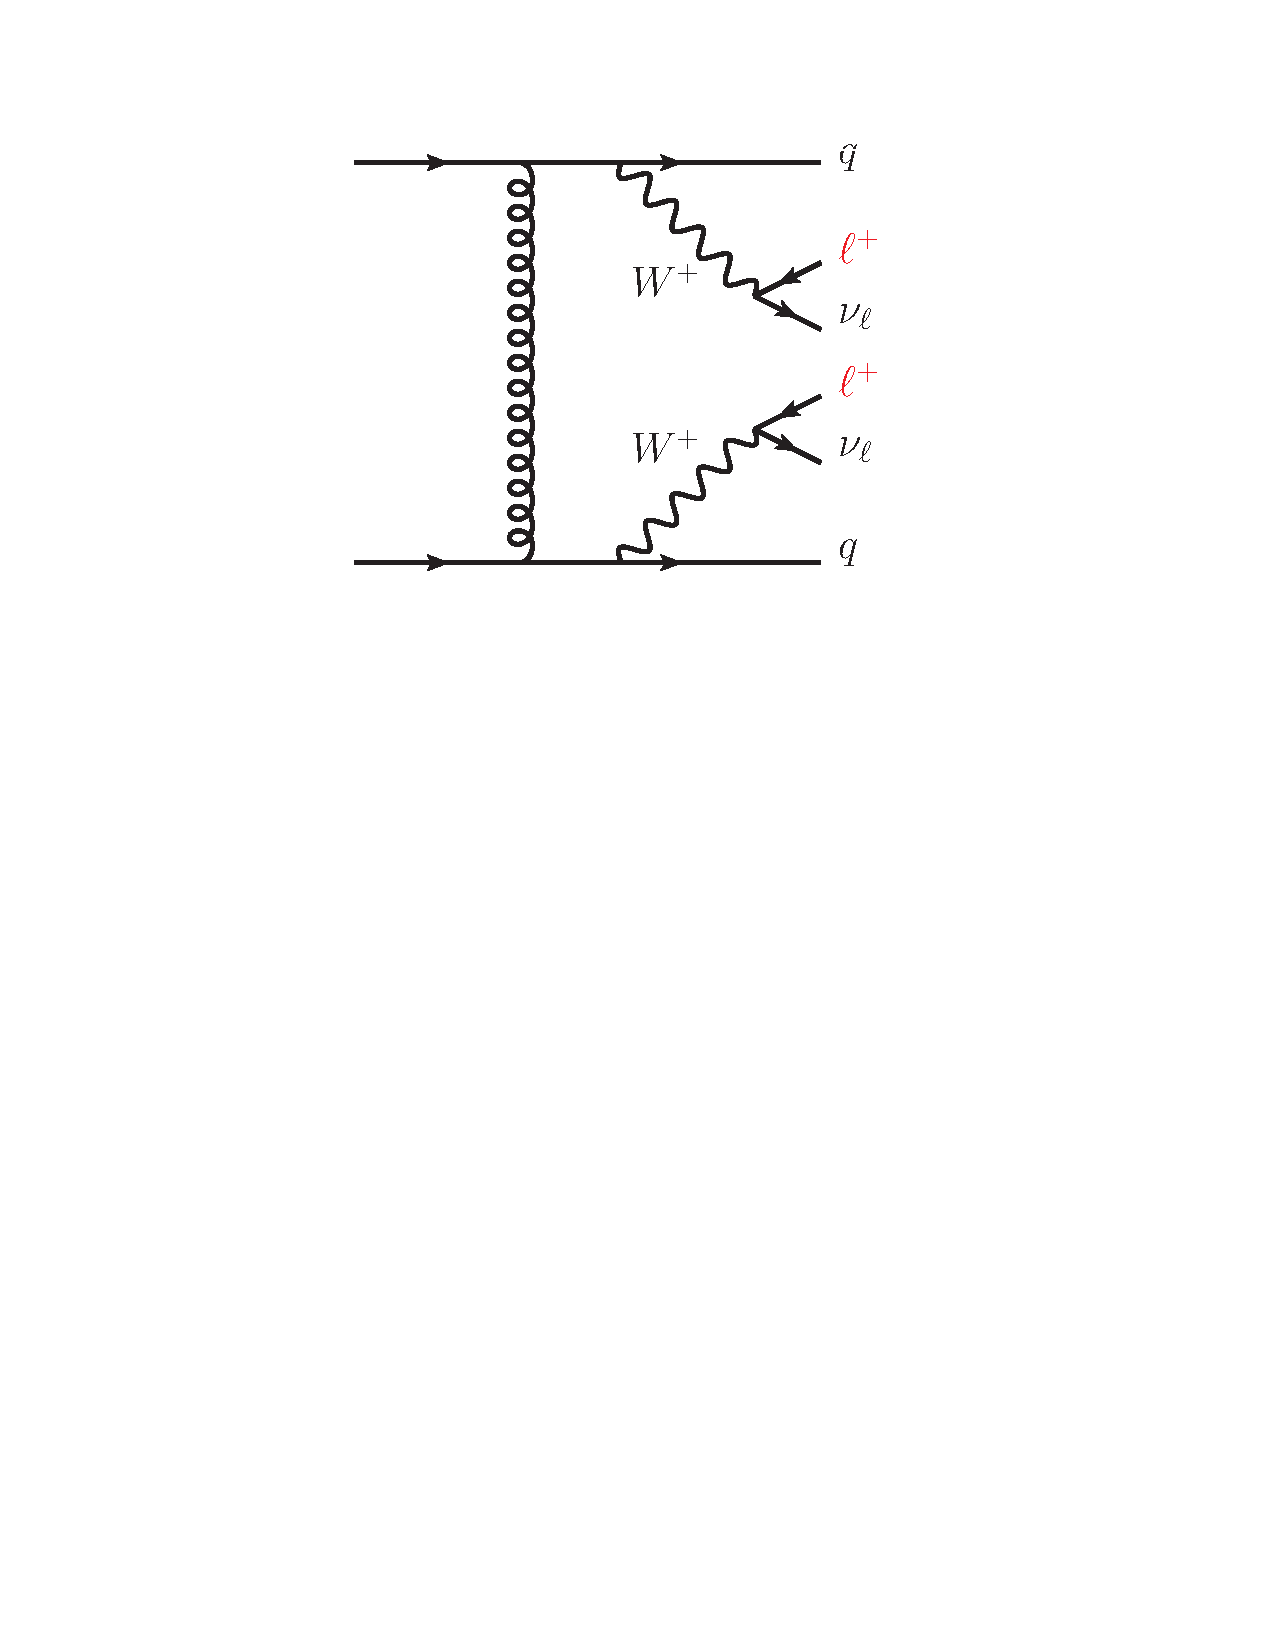
\includegraphics[width=0.8\textwidth, clip = true, trim = 1in 7.0in 1in 0.9in]{qqww.pdf}
\caption[Feynman diagram for \qqWW]
{\label{fig:feyn_ssww} 
Example leading order Feynman diagram for $\qqWW \to \ell^{\pm}\nu_{\ell}\ell^{\pm}\nu_{\ell} + qq$.
}
\end{center}
\end{figure}
% --------------------------------------------------------------------------- %
Processes than involve same-sign W pair production considered in this analysis are
listed below:
\begin{itemize}
\item \qqWW: Two same signed quarks are produced and each radiates a W boson which both decay leptonically ($pp \to qqWW$). 
\item \WWdps: Two independent hard parton collisions that both produce W bosons which both decay leptonically ($pp \to 2 \times \Wlnu$).
\end{itemize}

% --------------------------------------------------------------------------- %
% --------------------------------------------------------------------------- %
\section{Other Sources of Backgrounds}
\label{sec:ss_bkgd}
% --------------------------------------------------------------------------- %
% --------------------------------------------------------------------------- %
In the previous subsection, we discussed SM process that give rise to events
that posses genuine same-sign dileptons in the final state. In an ideal
scenario, this is all we would need to consider; however, there are two other
major sources of background that are caused by our inability to select the
correct events with 100\% certainty. The first of these is the non-negligible
situation when an electron or muon is reconstructed and mis-identified as a
prompt and isolated lepton. The second situation is less significant than the
first but nevertheless is still important and is accounted for. This is the
case where a real electron is reconstructed and selected; however, its electric
charge is mis-reconstructed. The following subsections will give a brief
discussion of these two cases, respectively.

% --------------------------------------------------------------------------- %
\subsection{Fake Leptons}
\label{sec:ss_bkgd_fakes}
% --------------------------------------------------------------------------- %

The dominant source of same-sign dileptons are events where one lepton is from
$\Wlnu$ and the other originates from a semi-leptonic b-quark decay. We refer
to leptons that originate from a electroweak boson or something with similar
properties (such as a super-symmetric object) as ``real leptons'' since these
give rise to true prompt and isolated leptons. For leptons that originate from
other sources, we refer to this as a ``fake lepton'' since this is not the
lepton we are interested in.

By far, the dominant source of fake leptons is $\ttbar$ events. A
representative diagram of this sort of event can be seen in the figure below
(Figure~\ref{fig:feyn_ttbar_fakes}).
% --------------------------------------------------------------------------- %
\begin{figure}[tbhp]
\begin{center}
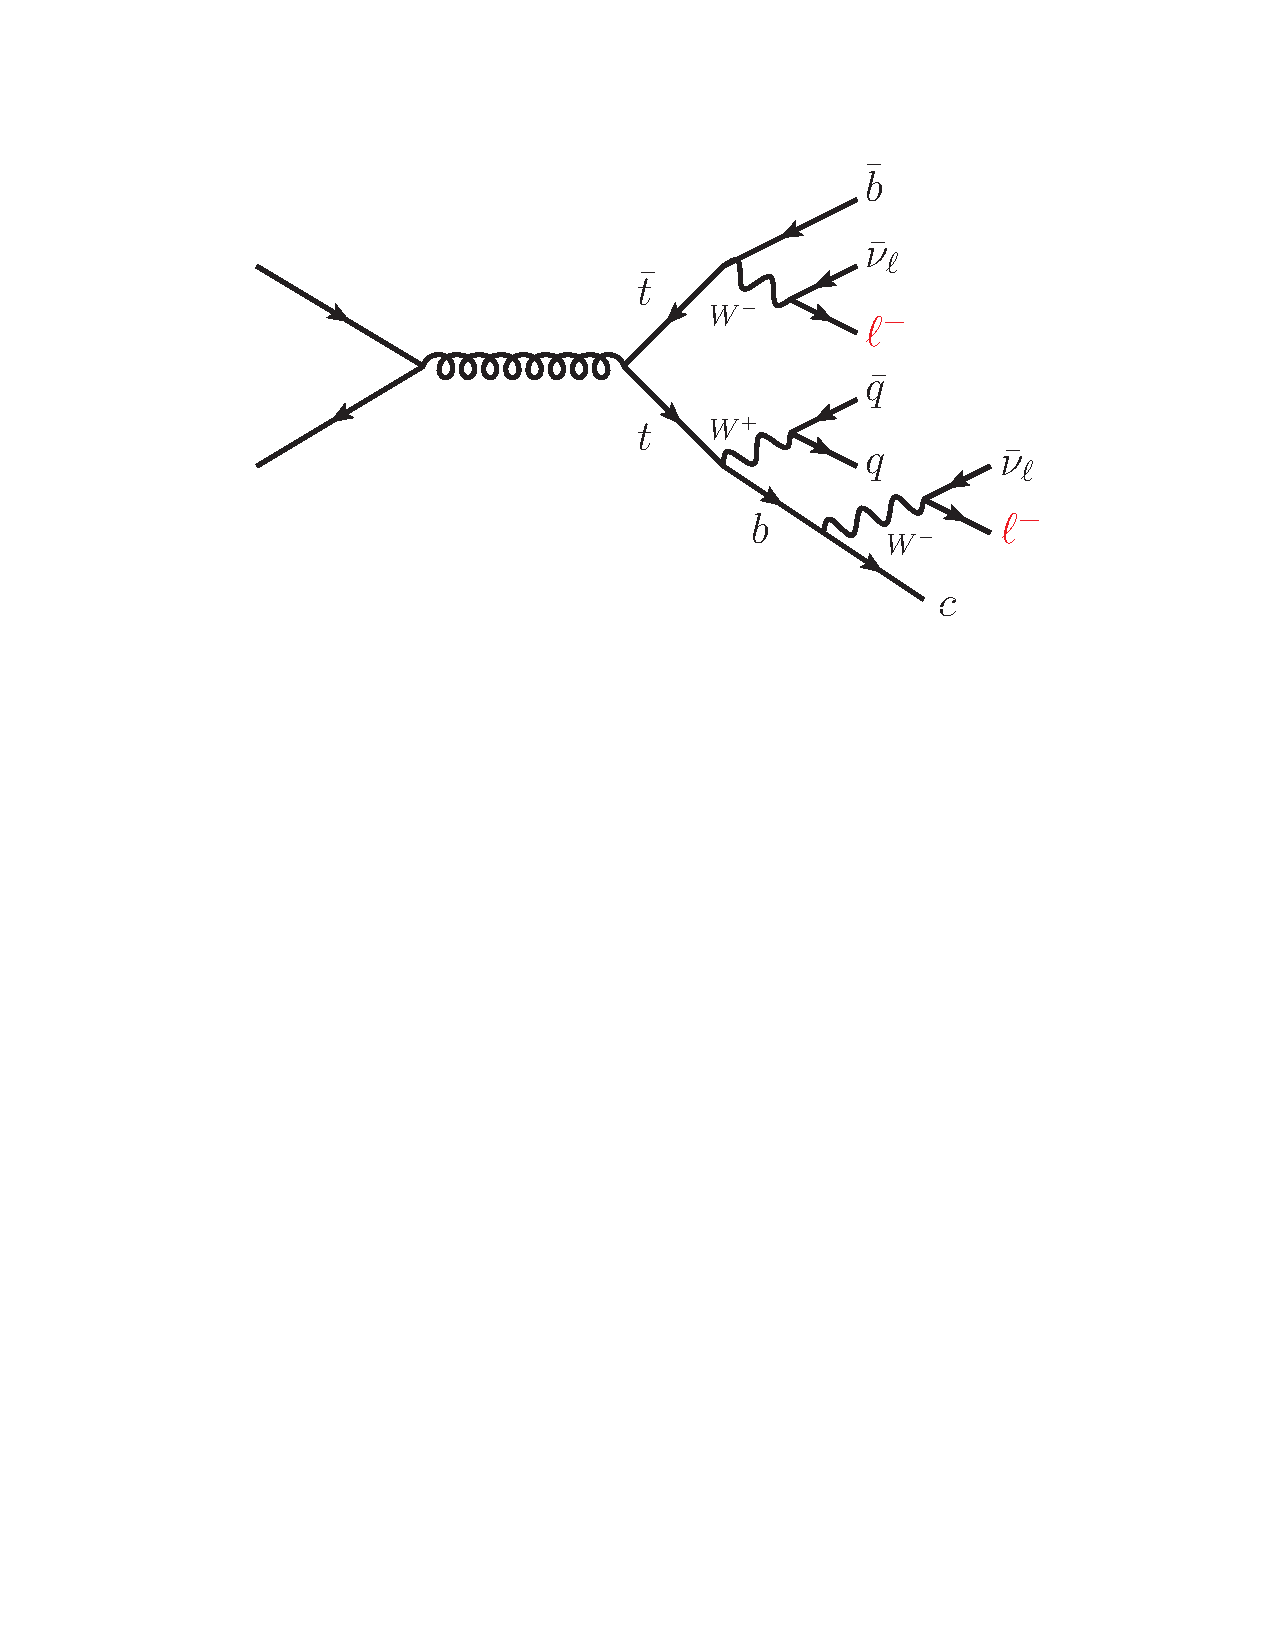
\includegraphics[width=0.8\textwidth, clip = true, trim = 1in 6.7in 1in 1in]{tt_fake.pdf}
\caption[Feynman diagram for fakes from \ttbar]
{\label{fig:feyn_ttbar_fakes} 
Diagram for \ttbar decays giving rise to same-sign dileptons final state.
}
\end{center}
\end{figure}
% --------------------------------------------------------------------------- %
Here we get a same-sign dilepton final state by having one of the leptons
from a top quark decaying leptonically from $\Wlnu$ and the other from
a ``fake'' lepton from the semi-leptonic b-quark decay from the other
top~\cite{an_ssb2011}. Anther important but sub-dominant source of fake lepton
background is from $pp \to \Wlnu + \text{jets}$ events where the jet decays
semi-leptonically.

The actual rate that the fake lepton will pass your analysis selection is
dependent on the details of the analysis. In Section \ref{sec:bkgd_fakes}, we
give a prediction on the number of same-sign dilepton event containing these
fake leptons.

% --------------------------------------------------------------------------- %
\subsection{Charge Flips}
\label{sec:ss_bkgd_flips}
% --------------------------------------------------------------------------- %

The measurement of a lepton's charge is determined from the curvature of the
reconstructed track as is travels through the magnetic field. The rate at which
the charge is mis-measured is negligibly small for muons at the W/Z momentum
scale; however, for electrons it is significant. Bremsstrahlung is emitted as
electrons are deflected by the silicon-based material of the track. A radiated
photon has a significant probability to covert into an \epem pair due to the
relatively large amount of material in the tracker~\cite{tdr1}. The combination
of the radiation of a hard photon and a subsequent asymmetric conversion (i.e.
when one of the two resulting electrons carries a significant fraction of the
momentum of the original photon) can result in the reconstruction of a track
that combines hits from the original electron with those from the converted
photon. As a result, the reconstructed track may have a curvature opposite to
that of the prompt electron, resulting in an incorrect charge assignment.

We estimate the rate that an electron that passes the analysis selection but
has an incorrect charge measurement to be $\sim 0.01\%$~\cite{an_ssb2013}.
The actual rate has been measured and will be fully discussed in Section
\ref{sec:bkgd_flips}.
